\chapter{ĐỐI TƯỢNG VÀ PHƯƠNG PHÁP NGHIÊN CỨU}

\textbf{
\section{Địa điểm và thời gian nghiên cứu}}
\qquad Địa điểm: Trường Đại học Y Dược - Đại học Quốc gia Hà Nội\par
\quad Thời gian nghiên cứu: Tháng 3 - tháng 5 năm 2023

\textbf{
\section{Đối tượng nghiên cứu}}
\subsection{Tiêu chuẩn lựa chọn đối tượng nghiên cứu:}
\qquad Sinh viên trong độ tuổi từ 18 – 25.\par
\quad Hàm răng tự nhiên, chưa được thực hiện các điều trị nha khoa trước đó như tẩy trắng răng, hàn răng hay hoặc răng giả, nắn chỉnh răng ....\par
\quad Có sức khỏe răng miệng tốt, không viêm lợi, không có cao răng mảng bám, không có  bệnh lý nội sinh và ngoại sinh ảnh hưởng đến màu sắc của răng.\par

\subsection{Tiêu chuẩn loại trừ:}
\begin{enumerate}
\setlength{\itemsep}{0pt}
    \item Người có vấn đề sức khỏe răng miệng nghiêm trọng: bệnh lý nha khoa nặng, viêm nhiễm hoặc sâu răng không điều trị.
    \item Đang được điều trị nha khoa liên quan đến màu sắc răng, chẳng hạn như tẩy trắng răng hoặc làm răng giả
    \item Những người có các yếu tố khác ảnh hưởng đến màu sắc răng, như hút thuốc lá, sử dụng các loại thức ăn, nước uống hoặc các biện pháp làm nhuộm màu răng như: cà phê, trà,...
    \item Bệnh nhân có tiền sử hoặc đang bị chấn thương răng dẫn đến thay đổi màu sắc răng.
    \item Không đồng thuận tham gia nghiên cứu hoặc không đáp ứng đầy đủ yêu cầu nghiên cứu, chẳng hạn như không hoàn thành câu hỏi khảo sát, không thực hiện các quy trình đo lường, hoặc không tuân thủ theo quy định và hướng dẫn của nghiên cứu.
\end{enumerate}
\vspace{-5pt}
\textbf{
\section{Phương pháp nghiên cứu}}
\quad Thiết kế nghiên cứu mô tả cắt ngang
\vspace{5pt}
\textbf{
\section{Phương pháp chọn mẫu}}
\quad Áp dụng công thức tính cỡ mẫu cho ước lượng một tỷ lệ:\par

\begin{equation*}
    \Large n = \mathrm{Z}_{1-\alpha/2}^{2}\frac{p(1-p)}{d^{2}}
\end{equation*}\par
%chèn công thức
\quad Trong đó:

\begin{itemize}[label={}, itemsep=-4pt]
    \item \textbf{n:} cỡ mẫu nghiên cứu cần có
    \item \textbf{p:} tỷ lệ răng có màu sáng theo Nguyễn Thị Châu (2013)\cite{NguyenThiChau} là 85\%
    \item \textbf{d:} khoảng sai lệch mong muốn tức tỷ lệ tuyệt đối được chúng tôi quy ước bằng 0,09
    \item \textbf{$\alpha$:} mức ý nghĩa thống kê được chúng tôi quy ước bằng 0.01 ứng với độ tin cậy 95\%  
    \item \textbf{$z^{2}_{1-\alpha/2}$:} giá trị Z tương ứng thu được bằng 1,96.
\end{itemize}

\par
\quad Thay vào công thức, có 
$n=1.96^{2}\times 0.85\times (1-0.85):0.09^{2}\approx 64$
\par  
\quad Cỡ mẫu tối thiểu cần cho điều tra nghiên cứu là 64 sinh viên, chúng tôi lấy 65.

\textbf{
\section{Quy trình tiến hành nghiên cứu}}
\subsection{Vật liệu và công cụ thu thập thông tin}
\qquad Bộ dụng cụ khám\par
\quad Ghế răng\par
\quad Bảng so màu Vita 3D\par

\begin{figure}  [h]
    \centering
    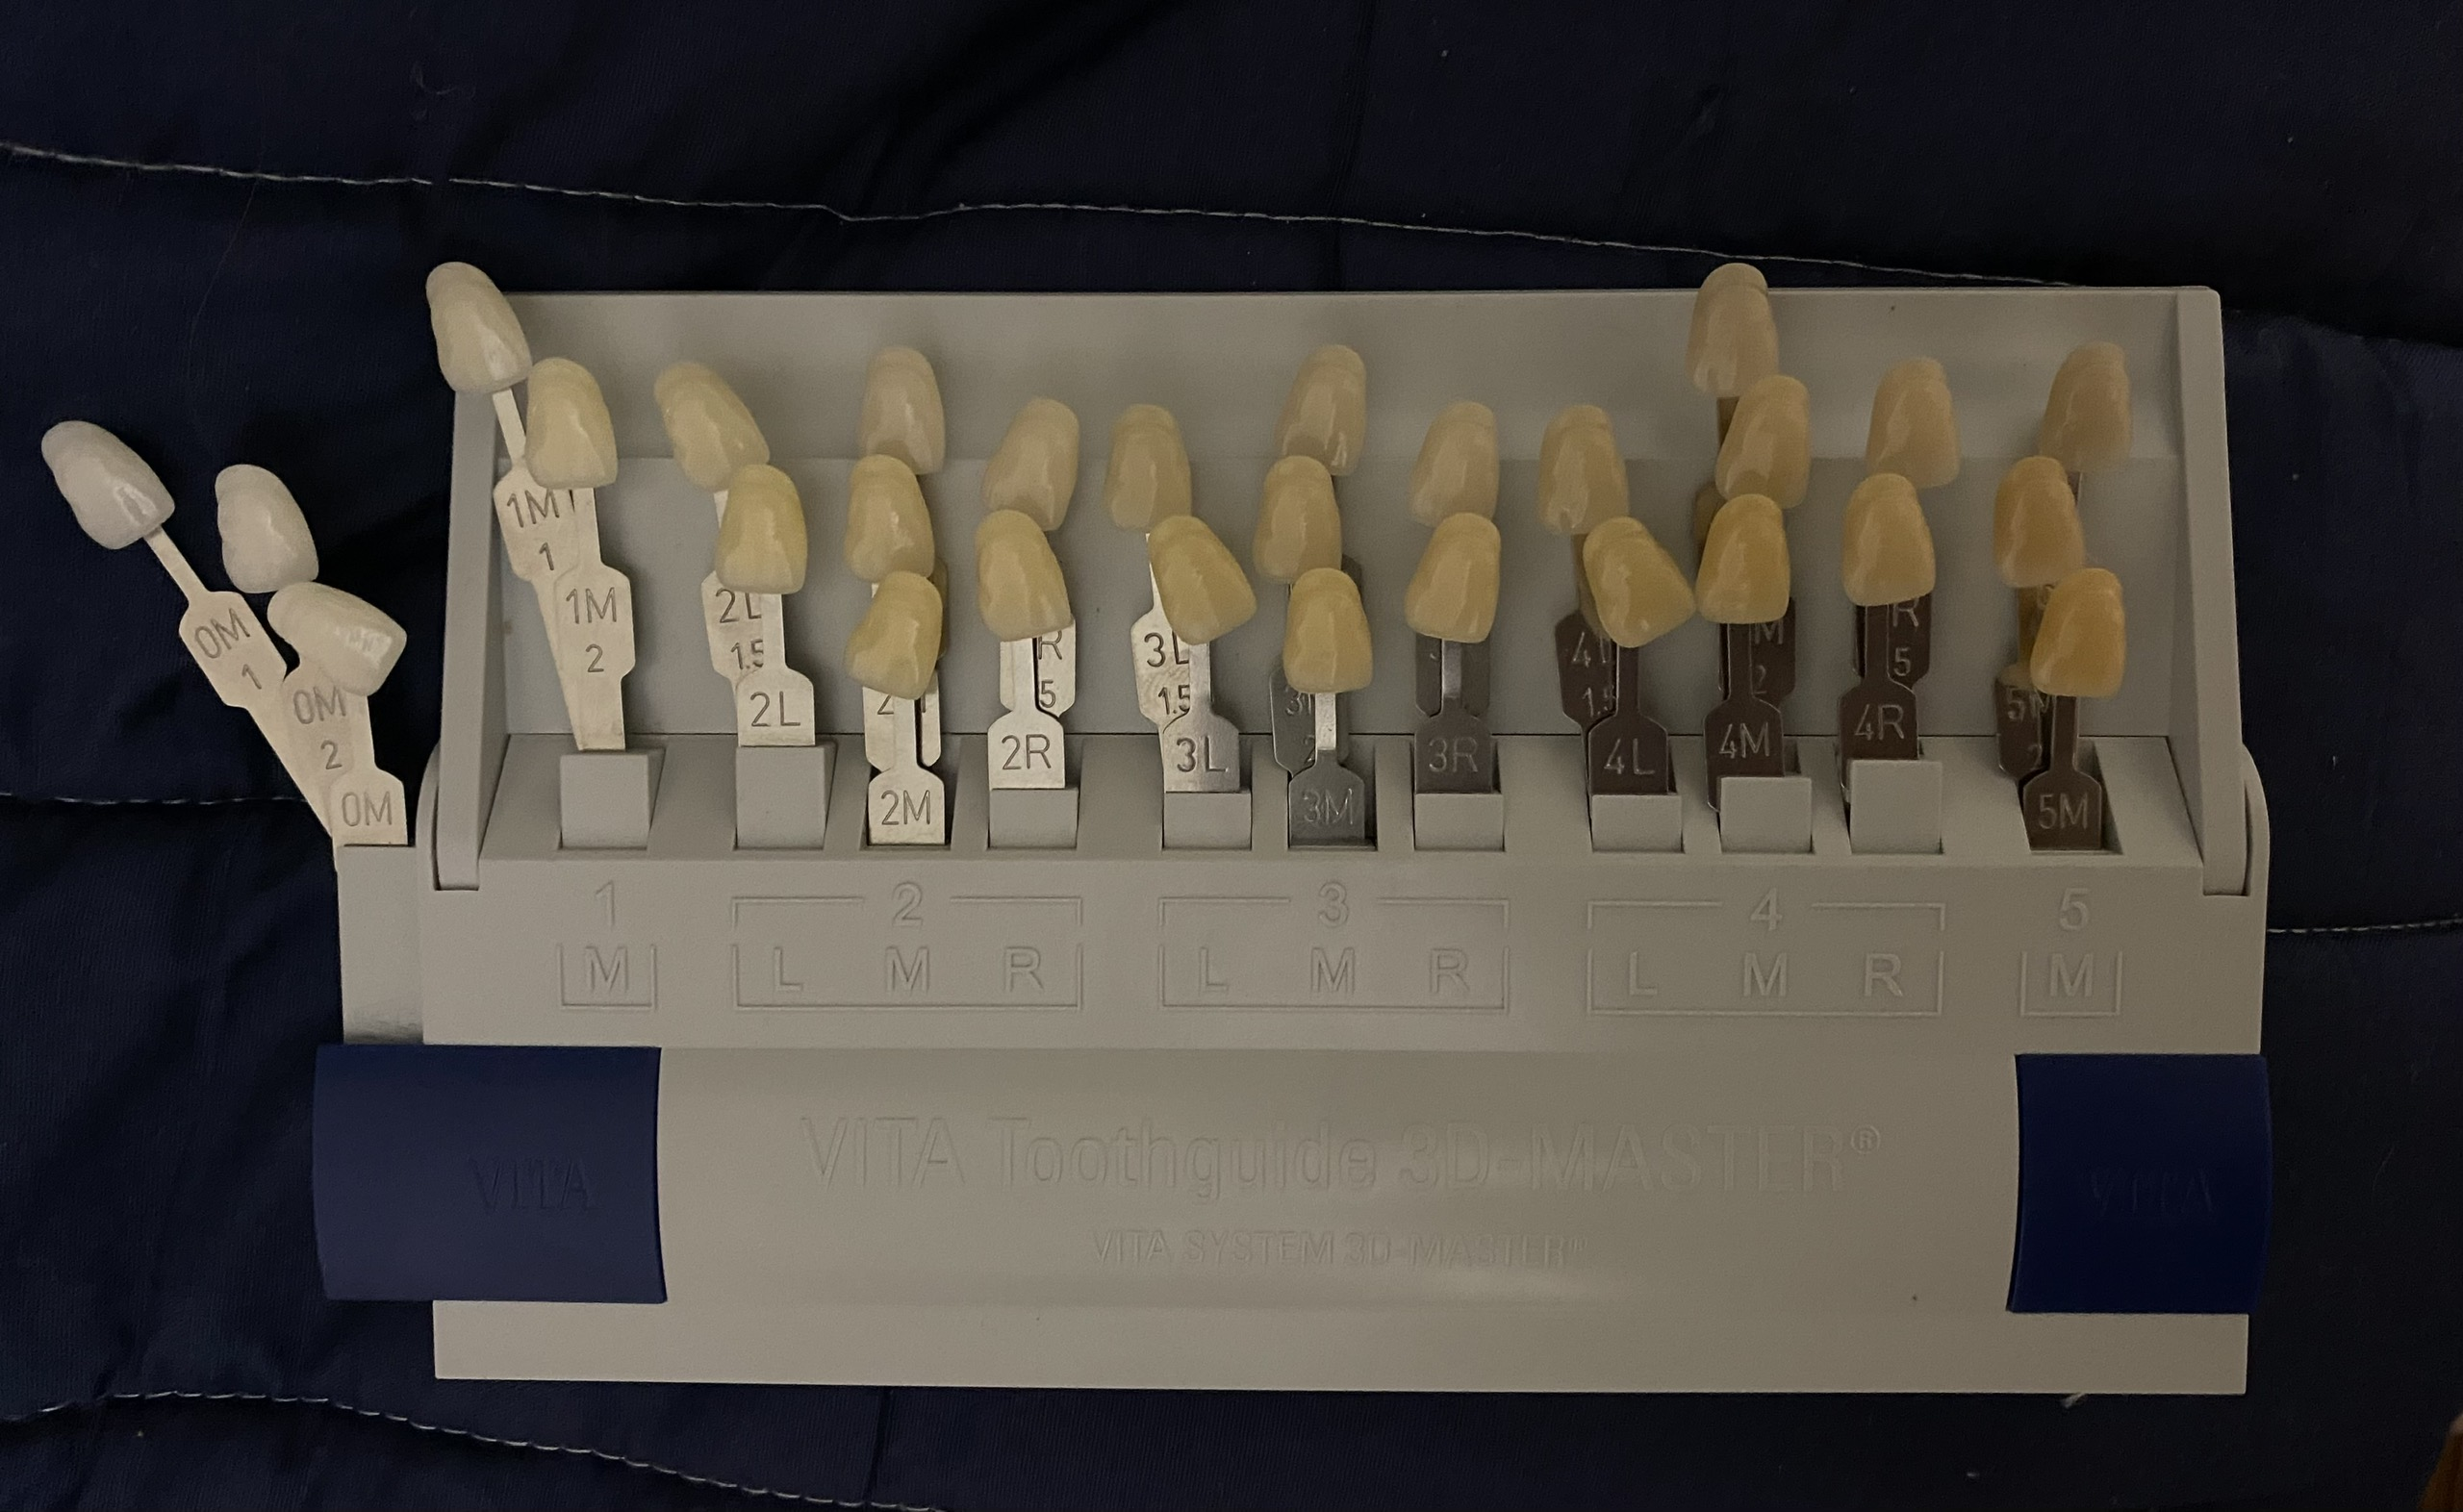
\includegraphics[width=0.7\columnwidth]{pictures/anh-bang-mau.jpeg}
    \caption {Ảnh bảng màu Vita 3D}
    \label{fig:anh-bang-mau}
    \end{figure}

\quad Bảng so màu Vita 3D được thiết kế theo ký hiệu theo thứ tự số - chữ cái - số (ví dụ 3M2), trong đó thể hiện theo thứ tự giá trị của Value, Chroma và Hue. Theo thứ tự value, chia thành 5 nhóm có giá trị value giảm dần từ nhóm 0 đến nhóm 5:\par
\quad Nhóm 0: Nhóm có value cao nhất, chỉ có một hue ký hiệu M (màu trung tính) có 3 cây 0M1, 0M2, 0M3 theo thứ tự tăng dần chroma từ nhạt đến sẫm màu hơn 0M1<0M2<0M3.\par
\quad Nhóm 1: 2 cây 1M1 và 1M2, có cùng hue màu trung tính ký hiệu M, có thứ tự tăng dần chroma 1M1<1M2.\par 
\quad Nhóm 2, 3 và 4: Có 7 cây, chia thành 3 phân nhóm nhỏ theo thứ tự thay đổi hue gồm: nhóm L (left) - màu vàng, nhóm M (medium) - màu trung tính, nhóm R (right) - màu đỏ. Trong nhóm L, độ chroma tăng dần 2L1<2L2; 3L1<3L2; 4L1<4L2. Trong nhóm M, độ chroma tăng dần 2M1<2M2<2M3; 3M1<3M2<3M3; 4M1<4M2<4M3. Trong nhóm R, độ chroma tăng dần 2R1<2R2; 3R1<3R2; 4R1<4R2.\par
\quad Nhóm 5: Có 3 cây, nhóm có value thấp nhất, chỉ có một hue ký hiệu M tương tự nhóm 0 (màu trung tính), 3 cây gồm 5M1, 5M2, 5M3 theo thứ tự tăng dần chroma 5M1<5M2<5M3.\par

\subsection{Lập phiếu thu thập thông tin}
\qquad Theo phụ lục 1

\subsection{Khám lâm sàng}
\textit{
\qquad Thực hiện so màu răng theo các bước sau:}\par
\begin{enumerate}
\setlength{\itemsep}{0pt}
\item Bước 1: Chọn value (Xác định độ sáng tối), chọn một trong năm nhóm sao cho độ sáng tối của răng giống nhất với độ sáng tối của các cây loại M trong bảng so màu từ nhóm value đã chọn được.
Giữ bảng so màu trên tay cạnh miệng bệnh nhân (đặt bên phải)
Chọn nhóm 0, 1, 2, 3, 4 hoặc 5 (0 là sáng nhất và 5 là tối nhất)
Bắt đầu so với với nhóm tối nhất trước.\par 
\item Bước 2: Chọn chroma (Chọn độ tương phản), dùng tông màu trung gian nhóm (M) để xác định độ tương phản bằng cách xòe que mẫu M như rẻ quạt. Chọn một trong ba màu sắc tương tự, gần giống nhất với răng được so màu.\par 
\item Bước 3: Chọn tông màu hue ( Kiểm trả xem răng tự nhiên vàng (bên trái L), trung tính (M) hay đỏ (bên phải R) hơn so với bảng màu: so sánh với các cây loại L và R có cùng nhóm với  cây loại M vừa chọn (cùng độ value và chroma), từ đó chọn ra cây có hue gần giống nhất với răng so màu, viết ký hiệu màu chọn theo quy ước của bảng so màu.\par 
\end{enumerate}
\textit{
\qquad So màu răng tuân thủ theo nguyên tắc sau đây:}\par 
\begin{itemize}
\setlength{\itemsep}{0pt}
    \item Đảm bảo đủ tiêu chuẩn về nguồn sáng, dùng ánh sáng hiệu chỉnh (color-corrected lighting) với nhiệt độ màu từ 5500 (D55) - 6500K (D65), chỉ số hoàn màu (color-rendering index) >=90; độ rọi (illuminance) từ 1000 đến 2000 lux, lý tưởng nhất dưới ánh sáng tự nhiên và đủ tiêu chuẩn kỹ thuật trên. Loại bỏ màu sắc gây nhiễu xung quanh răng so màu như son môi, đèn chiếu sáng khác, nên dùng nền tường không gian so màu là màu xám nhạt, tránh sử dụng màu sắc khác gây nhiễu loạn và mỏi mắt trước và trong khi so màu.\par 
\item Khi so màu, mắt người so màu để ngang mức răng, khoảng cách từ răng đến mắt khoảng từ 25-35cm (tương ứng 10-14 inch). Góc chiếu sáng và góc nhìn của người so màu phù hợp nhất là 45 độ/0 độ hoặc 0 độ/45 độ; mắt người quan sát thường ở vị trí trung tâm và nguồn chiếu sáng từ 1 hướng, 2 hướng và xung quanh.\par
\item Răng so màu cần được làm sạch, để ở trạng thái tự nhiên, không quá khô hoặc không quá ướt. Thời gian so màu từ 5-7 giây để tránh mỏi mắt và quen màu, tránh nhìn liên tục và cần cho mắt nghỉ ngơi, thời gian nghỉ ngơi tối thiểu là 5 phút, nên nhìn vào màu xám nhạt khi thư giãn mắt giữa những lần so màu.\par 
\item Vị trí đặt bảng so màu phụ thuộc vào phương pháp so màu và mục đích so màu, so màu pha macro thì đặt bảng so màu, sau đó chọn các cây tiếp tục cho pha sau như pha mini và pha micro.\par 
\item Đặt giữa răng hàm trên và hàm dưới hoặc kế bên ngang mức rìa cắn răng cần so màu, tránh đặt chồng lên phía trước hoặc phía sau răng cần so màu:\par 
\begin{itemize}
\setlength{\itemsep}{0pt}
\item Đặt đối đầu (rìa cắn - rìa cắn): Để so màu rìa cắn, nhưng không thể so màu cổ và thân răng.
\item Đặt cổ - rìa cắn: ít khi thực hiện.
\item Đặt nằm ngang: Để so màu thân răng.
\end{itemize}\par
\item Nếu đặt cây so màu bên cạnh răng cần so thì phải nghiêng tạo thành một góc 120 độ so với bề mặt răng thật, và quan sát từ hướng phân giác của góc này đến hai bề mặt răng thật và răng trên bảng so màu.\par 
\item Phương pháp so màu theo mô hình ba pha macro - mini - micro, bắt đầu bằng pha macro bằng cách sử dụng toàn bộ bảng so màu, chọn và đặt sang một bên các màu được lựa chọn để dùng cho pha sau, loại bỏ các màu không phù hợp. Ở pha mini, các cây được lựa chọn thì chọn tiếp sao cho phù hợp về màu của cổ, thân và rìa cắn gần nhất với răng cần so màu. Ở pha micro thì so sánh chi tiết về hue, value và chroma. Không đặt rìa cắn hướng về phía kim loại của bảng so màu.\par 
\item Nên so màu răng cả cùi răng và so màu từng phần của răng thành ba phần rìa cắn, thân và cổ răng. Nên thay đổi thêm góc độ để quan sát màu và nếu khó khăn trong việc quyết định màu thì nên mời thêm những chuyên gia khác cùng so màu và đưa ra kết luận chung một cách khách quan. Kết quả so màu cần ghi ký hiệu màu dưới dạng “ngôn ngữ màu (color language)” theo từng loại bảng so màu của nhà sản xuất nhằm thống nhất màu giữa bác sĩ và labo răng.\par 
\item Chụp hình màu được chọn nhằm tăng thêm dữ liệu đáng tin cậy cho sự giao tiếp màu giữa bác sĩ và labo, bác sĩ cần chụp ảnh kèm thêm hai màu gần nhất với màu được chọn đặt ở giữa so với hai màu lân cận (một màu sáng và một màu tối hơn so với màu được chọn). Đèn flash để chụp ảnh cần đảm bảo trong khoảng nhiệt trung tính (khoảng 5500K) để màu hình ảnh tự nhiên.\par

\end{itemize}

\vspace{-5pt}
\textbf{
\section{ Biến số, chỉ số nghiên cứu}}
\noindent
\textbf{Mục tiêu 1: Mô tả thực trạng nhiễm màu răng ở sinh viên trường đại học Y dược - Đại học Quốc gia Hà Nội năm 2023}

%chèn bảng biến số vô đây
\begin{longtable}{|l|l|l|l|l|} 
\hline
\textbf{STT} & \textbf{Biến số} & \textbf{Loại biến số} & \textbf{Định nghĩa biến} & \textbf{Phân tích}  \endfirsthead 
\hline
1            & Giới             & Định tính             & Nam hay nữ               & Tính tỷ lệ \%       \\ 
\hline
2            & Tuổi             & Định lượng            & Số tuổi                  & Tính tỷ lệ \%       \\ 
\hline
3            & Màu sắc răng     & Định tính             & Màu sắc răng             & Tính tỷ lệ \%       \\
\hline
\end{longtable}
\noindent
\textbf{Mục tiêu 2: Xác định nhu cầu điều trị ở nhóm đối tượng trên}

%chèn bảng biến số tiếp
\begin{longtblr}[
  label = none,
  entry = none,
]{
  width = \linewidth,
  colspec = {Q[54]Q[265]Q[138]Q[340]Q[127]},
  hlines,
  vlines,
}
\textbf{STT} & \textbf{Biến số}           & \textbf{Loại biến số} & \textbf{Định nghĩa biến}        & \textbf{Phân tích} \\
1            & Sự đổi màu răng            & Định tính             & Mức độ đổi màu răng             & Tính tỷ lệ \%      \\
2            & Vị trí phân bố đổi màu sắc & Định tính             & Vị trí phân bố vết đổi màu      & Tính tỷ lệ \%      \\
3            & Ảnh hưởng tới người bệnh   & Định tính~            & Mức độ ảnh hưởng tới người bệnh & Tính tỷ lệ \%      \\
4            & Nhu cầu làm trắng răng     & Định tính             & Nhu cầu làm trắng răng          & Tính tỷ lệ \%      
\end{longtblr}

\textbf{
\section{Đánh giá chỉ số nhu cầu làm trắng răng}}
\quad Chỉ số nhu cầu điều trị làm trắng răng được đánh giá theo Linda Greenwall như sau:\par
\noindent
\textbf{Loại 1 - Cao}
\begin{enumerate}
\setlength{\itemsep}{0pt}
    \item Sự đổi màu: nghiêm trọng
    \item Vị trí vết: phân bố nhiều đậm nhạt đồng đều
    \item Ảnh hưởng đến trẻ em: nghiêm trọng
    \item Nhu cầu làm trắng: cao
\end{enumerate}
\noindent
\textbf{Loại 2 - Trung bình}
\begin{enumerate}
\setlength{\itemsep}{0pt}
    \item Sự đổi màu: vừa phải
    \item Vị trí: phân bố đều
    \item Ảnh hưởng đến đứa trẻ: có ảnh hưởng đến đứa trẻ
    \item Nhu cầu làm trắng: vừa phải
\end{enumerate}
\noindent
\textbf{Loại 3 — Mong muốn}
\begin{enumerate}
\setlength{\itemsep}{0pt}
    \item Sự đổi màu: nhẹ
    \item Vị trí: ít răng trước
    \item Tác động đến trẻ em: một số tác động
    \item Nhu cầu làm trắng: mong muốn; điều này sẽ dễ dàng làm giảm bớt các vấn đề đổi màu
\end{enumerate}
\noindent
\textbf{Loại 4 — Khuyến cáo}
\begin{enumerate}
\setlength{\itemsep}{0pt}
    \item Sự đổi màu: các khu vực bị đổi màu bị cô lập
    \item Vị trí: phân bố ngẫu nhiên trên răng
    \item Ảnh hưởng đến trẻ em: vừa phải
    \item Nhu cầu làm trắng: khuyến cáo
\end{enumerate}
\noindent
\textbf{Loại 5 — Có thể}
\begin{enumerate}
\setlength{\itemsep}{0pt}
    \item Sự đổi màu: đổi màu nhẹ hoặc đốm trắng
    \item Vị trí: ít răng hoặc một răng
    \item Ảnh hưởng đến trẻ em: không ảnh hưởng đến trẻ em
    \item Nhu cầu làm trắng: có thể thực hiện được; có thể được mong muốn, nhưng có thể đợi cho đến khi đứa trẻ trên 18 tuổi.
\end{enumerate}

\vspace{-5pt}
\textbf{
\section{Thu thập dữ liệu}}
\quad Số liệu thu thập và phân tích bằng phương pháp thống kê y học, sử dụng phần mềm SPSS, Excel.\par
\quad Với mục tiêu 1 và 2: Mô tả đặc điểm màu sắc răng theo bảng màu Vita 3D Master và đánh giá nhu cầu làm trắng răng ở người bệnh: số liệu được trình bày bằng các bảng tần suất và các biểu đồ phù hợp.\par

\textbf{
\section{Đạo đức nghiên cứu}}
\quad Nghiên cứu được tiến hành khi hội đồng chấm đề cương thông qua và được sự đồng ý của Ban Giám Hiệu Trường Đại học Y Dược - Đại học Quốc gia Hà Nội.\par	
\quad Trước khi tiến hành nghiên cứu, giải thích đầy đủ cặn kẽ, chu đáo cho các người bệnh tham gia nghiên cứu. Người bệnh chấp thuận tham gia nghiên cứu và tự nguyện ký vào bản tham gia nghiên cứu.	\par
\quad Các thông tin thu thập được giữ bí mật, chỉ dùng với mục đích nghiên cứu. Nghiên cứu nhằm cải thiện thẩm mỹ và bảo vệ chăm sóc sức khỏe cho bệnh nhân mà không nhằm vào mục đích khác. \par
\vspace{-5pt}
\textbf{
\section{Sai số và biện pháp tránh sai số}}
\quad Khi so màu răng, có thể xảy ra sai số do nhiều yếu tố khác nhau như ánh sáng, góc nhìn, màu sắc tham chiếu và sự chủ quan của người quan sát. Tuyệt đối không thể loại trừ hoàn toàn sai số khi so màu răng, nhưng bằng cách tuân thủ những một số nguyên tắc sau giúp giảm sai số và đạt được kết quả gần đúng nhất trong quá trình so màu. để hạn chế sai số chúng tôi thực hiện như sau:\par
\quad Sử dụng điều kiện ánh sáng chuẩn: Đảm bảo răng được so màu trong điều kiện ánh sáng tự nhiên hoặc ánh sáng có màu sắc và cường độ đồng nhất. Tránh ánh sáng mạnh quá mức hoặc ánh sáng có màu sắc biến đổi có thể ảnh hưởng đến quá trình so màu.\par
\quad Đảm bảo môi trường không màu nhiễu: Tránh môi trường có màu sắc nổi bật hoặc quá phức tạp, vì nó có thể gây nhiễu và ảnh hưởng đến quá trình so màu. \par
\quad Một phòng chụp màu riêng biệt hoặc môi trường có màu trung lập có thể được sử dụng để giảm sai số.\par
\quad Sử dụng màu chuẩn ổn định: Chọn một bảng màu chuẩn hoặc màu sắc tham chiếu ổn định và được công nhận trong ngành nha khoa. Đảm bảo rằng màu chuẩn không bị mờ hoặc thay đổi màu theo thời gian.\par
\quad Đo và ghi lại màu sắc theo cách chuẩn: Sử dụng thiết bị đo màu nếu có thể để có kết quả chính xác và đáng tin cậy. Nếu sử dụng mắt thường, hãy cố gắng đánh giá màu sắc từ nhiều góc độ và so sánh với màu chuẩn càng cẩn thận càng tốt. Ghi lại màu sắc một cách chính xác và chi tiết để có thể so sánh và theo dõi sự thay đổi màu theo thời gian.\par
\quad Người so màu được huấn luyện về cách so màu so màu răng để giảm sai số. cần có thể có những kỹ năng và kinh nghiệm cần thiết để nhận biết và đánh giá màu sắc răng một cách chính xác.\par
\quad Kiểm tra lại kết quả với đánh giá thứ 2 và thảo luận: Kiểm tra lại kết quả so màu và thảo luận với người đánh giá thứ 2 để đảm bảo tính chính xác và đáng tin cậy của quá trình so màu.\par


